\documentclass[
	ngerman,
	xcolor=dvipsnames,
	11pt
	]{beamer}
\usepackage{babel}
\usepackage[utf8]{inputenc}
\usepackage[LY1]{fontenc}
\renewcommand{\rmdefault}{NexusSerifPro}
\renewcommand{\sfdefault}{NexusSansPro}
%\usepackage{soul}	%\textst command
\usepackage{ulem} 	%\uline \sout \xout \uuline \uwave

\usepackage{tikz}
\usetikzlibrary{arrows,calc}
\tikzset{
%Define standard arrow tip
>=stealth',
%Define style for different line styles
help lines/.style={dashed, thick},
axis/.style={<->},
important line/.style={thick},
connection/.style={thick, dotted},
}

\newcommand{\beginbackup}{
   \newcounter{framenumbervorappendix}
   \setcounter{framenumbervorappendix}{\value{framenumber}}
}
\newcommand{\backupend}{
   \addtocounter{framenumbervorappendix}{-\value{framenumber}}
   \addtocounter{framenumber}{\value{framenumbervorappendix}} 
}

\setbeamertemplate{navigation symbols}{}

%% TUBS
\usetheme[pageofpages=von,% page count separator
          tulogo=tubs,
			 institutelogo=ida]
			 {TUBS}
\usecolortheme{tubs}

\title[SEP 2011]{Simualtion von Achterbahnen}
\subtitle{SEP 2011}
\author{\tiny{Matthias Christian Daniel Simon  Robin Konstantin Marco}}
\institute[TU-BS]{Technische Universit"at Carolo-Wilhelmina zu Braunschweig}
\date{25.05.2011}

%\AtBeginSubsection[]
%{
%  \begin{frame}<beamer>
%    \frametitle{Layout}
%    \tableofcontents[currentsection,currentsubsection]
%  \end{frame}
%}

\newenvironment{annot}{\begin{block}{}}{\end{block}}

\begin{document}

	\begin{frame}
		\titlepage
	\end{frame}
	
	
	\section{Zielsetzungen}
	\begin{frame}{Zielsetzungen}
	\begin{itemize}
	\item Ingenieursm"a"sige Konstruktion einer Achterbahn
		\begin{itemize}
			\item Physikalisch korrekte Berechnung: Newtonsche Mechanik
			\item Ad"aquate Visualierung: 2 parallele Schienen, Quertr"ager, Bodenfl"ache
			\item Darstellung der Bahnparamter: Beschleunigung "uber Zeit etc.
		\end{itemize}
		
	\end{itemize}

	\end{frame}
	
	

	
	%\subsection{Vorschau}
	\begin{frame}{Visualisierung: Vorschau}
		\begin{figure}
			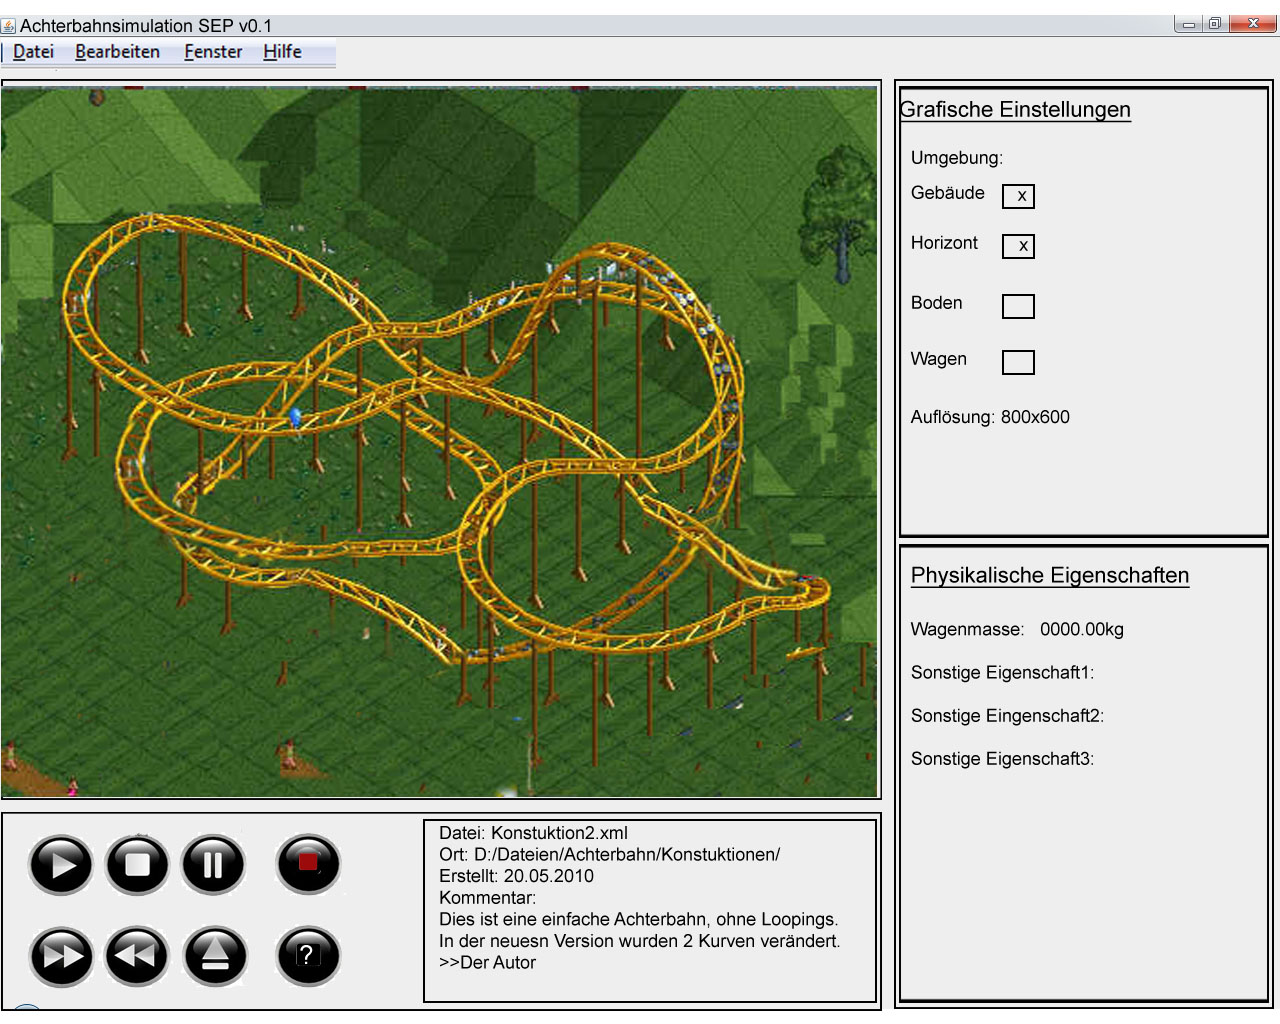
\includegraphics[width=0.78\linewidth]{GUI_v3.jpg}
		\end{figure}
	\end{frame}
	
	%\subsection{Fahrt}
		\begin{frame}{Visualisierung: Fahrt}
		\begin{figure}
			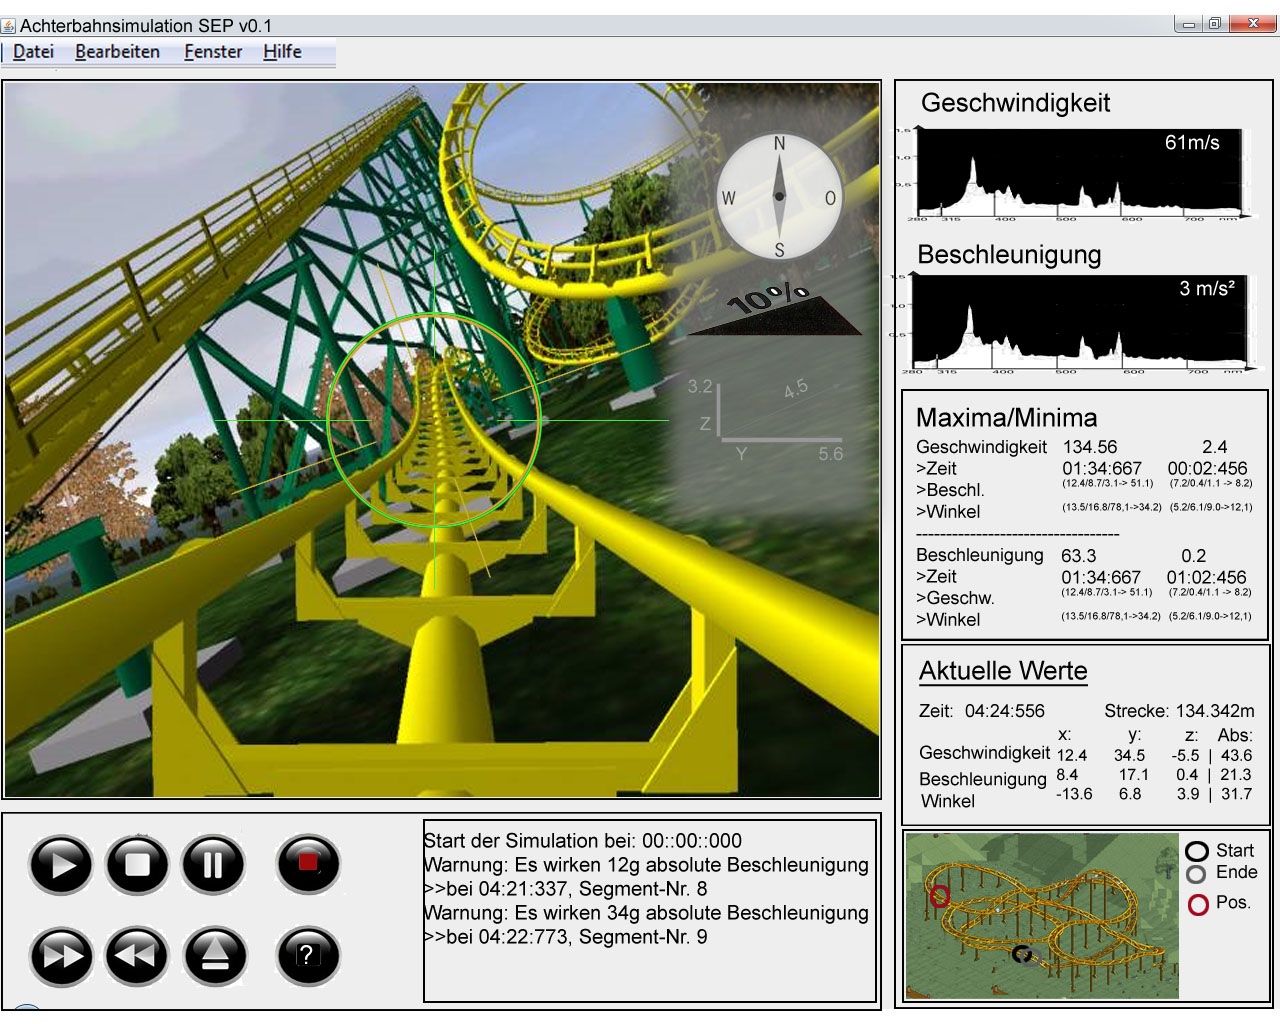
\includegraphics[width=0.78\linewidth]{GUI_v2.jpg}
		\end{figure}
	\end{frame}
	
	\section{Komponenten}
	\begin{frame}{Komponenten}
		\begin{figure}
			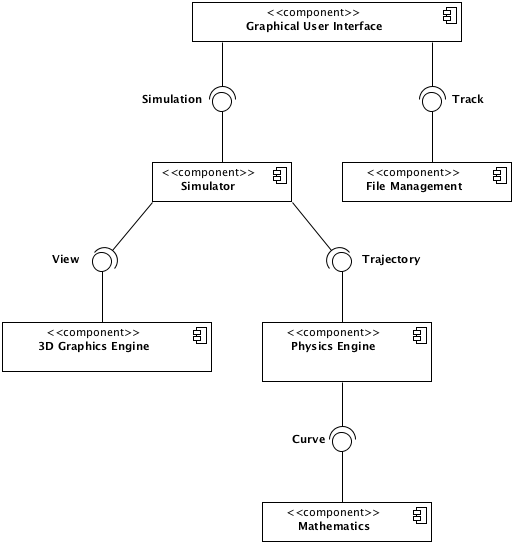
\includegraphics[width=0.55\linewidth]{component_overview.png}
		\end{figure}
	\end{frame}
	
	
\end{document}
